\subsubsection{Coherent Population Trapping (CPT)}
\label{sssec:CPT}

In case of a \acrfull{cpt} based system, the \acrshort{pp} contains a vapor gas cell that receive a high energy signal from a laser source and force the valence electron of the \acrfull{cs} atoms to a coherent superposition of the two hyperfine ground states.
If this coherent superposition happens, the electron is said to be \textit{trapped in a dark state}, given that the incoming laser source will no more be coupled with the electron transitions and the atoms will not absorb the photons.

Similarly to the \acrshort{modr}, by measuring the intensity of the transmitted light, we can understand if the local oscillator was in resonance with the atomic transition or not.

% In a \acrshort{pp} based on \acrshort{cpt}, a vapor gas cell is irradiated by a highly modulated-circularly polarized laser source.
% The laser source is modulated based on the local oscillator frequency.
% Based on the effect of the laser source on the \acrfull{cs} atoms, we can understand whether the local oscillator is in resonance with the atomic transition frequency or not.

In order to better visualize the operation of a CPT-based \acrshort{csac}, we leave here a schematic representation of its PP (Figure \ref{fig:CPT-physics-package-scheme}).

\begin{figure}[H]
    \centering
    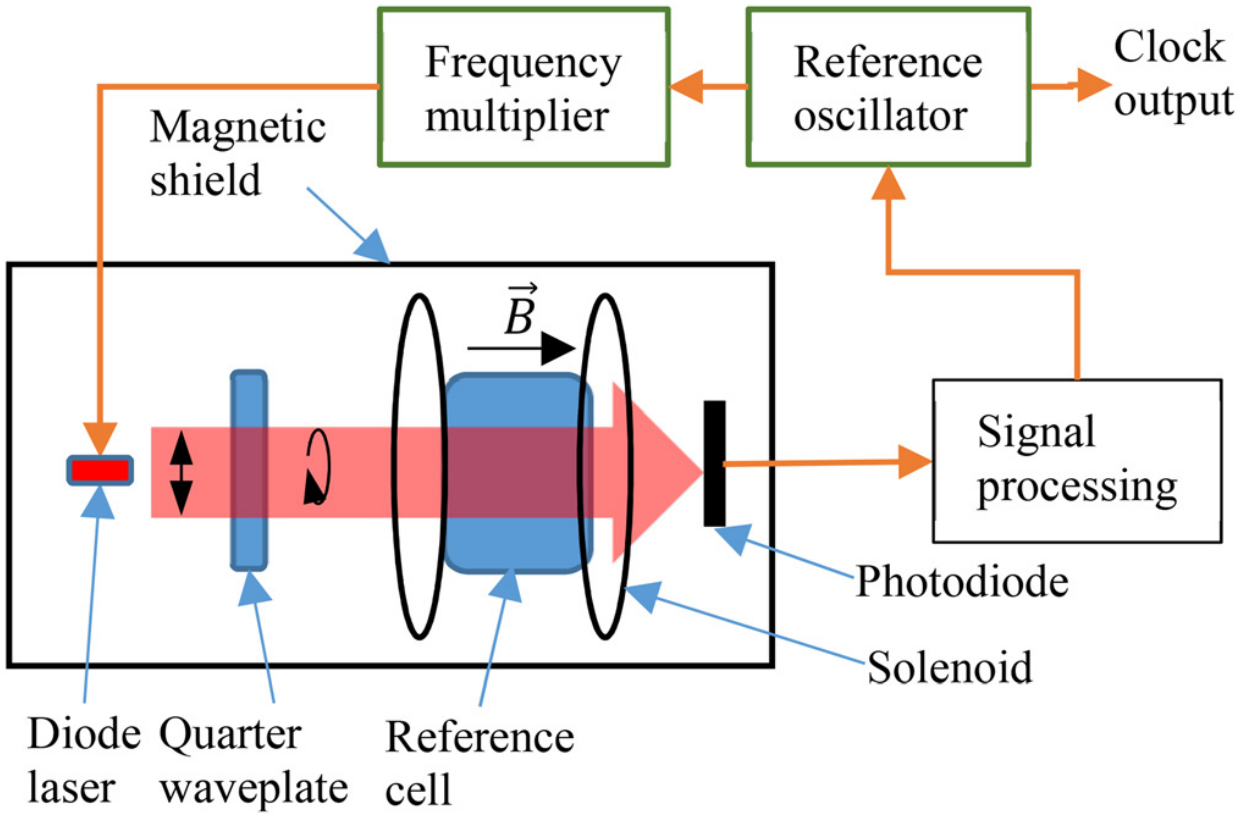
\includegraphics[width=0.6\textwidth, max width=\linewidth]{img/CPT-phisics-package-scheme.png}
    \caption{
        CPT-based \acrshort{csac} scheme.
        Source \cite{Kitching-2018}.
    }
    \label{fig:CPT-physics-package-scheme}
\end{figure}


\paragraph{Target Electron Transitions of Cesium (Cs)}

In case of PP based on CPT, the vapor gas cell is typically filled with \acrfull{cs} ($^{133}Cs$) atoms.
$Cs$ is an alkaline metal with a relatively simple electronic structure, defined as $[Xe]6s^1$.
Its first ionization energy is $3.894 eV$, and the valence electron can be exited using relatively low energy photons.
For these reasons, $Cs$ is widely used in atomic clocks, as it allows for precise manipulation of the valence electron while containing the energy required for the excitation.

In particular, by recalling the quantum energy levels of $^{133}Cs$ (defined by quantum effects and interactions between the electron and the nucleus), we can better define our working frame for the CPT architecture.
Three different transitions are of interest regarding the $^{133}Cs$ atom\footnote{A more comprehensive analysis of the $6S$ \& $6P$ energy levels of $^{133}Cs$ can be found in the Appendix \ref{appendix:Cesium-energy-levels}.}:

\begin{enumerate}[label = Cs.\Roman*, ref = Cs.\Roman*, leftmargin = *]
    \item \label{itm:Cs-I} $6^2S_{1/2} \quad F=3 \rightarrow 6^2S_{1/2} \quad F=4$: $\approx 9.2GHz$
    \item \label{itm:Cs-II} $6^2S_{1/2} \quad F=3 \rightarrow 6^2P_{1/2}$: $\approx 895^{-}nm$
    \item \label{itm:Cs-III} $6^2S_{1/2} \quad F=4 \rightarrow 6^2P_{1/2}$: $\approx 895^{+}nm$
\end{enumerate}

Notice that the transition $6^2S_{1/2} \rightarrow 6^2P_{1/2}$, of $\approx 895nm$, is usually refereed to as \textit{D1 line}.


\paragraph{Quantum Superposition}

Before moving on and understanding the different components of the CPT-based \acrshort{csac}, it's important to understand the concept of quantum superposition as it will be the key in the operation of the system.

In quantum mechanics, a quantum superposition is a fundamental principle that states that linear combinations of solutions to the Schr\"{o}dinger equation are also solutions of the equation itself.
In other words, if $\ket{\psi_1}$ and $\ket{\psi_2}$ are solutions of the Schr\"{o}dinger equation, then $\alpha\ket{\psi_1} + \beta\ket{\psi_2}$ is also a valid solution of the state of the system.
A valid quantum superposition can be generally defined as:

\begin{equation}
    \ket{\psi} = c_\alpha\ket{\psi_\alpha} + c_\beta\ket{\psi_\beta}
\end{equation}

Where $\ket{\psi_\alpha}$ and $\ket{\psi_\beta}$ are two different energy configurations of the system and $c_\alpha$ and $c_\beta$ are complex numbers.
Practically speaking, this means that the electron can be found not only in $\ket{\psi_\alpha}$ or $\ket{\psi_\beta}$, but also in any a superposition of the two states (with a probability defined by the complex numbers).

To facilitate the understanding of this counterintuitive concept, we report two different interpretations of the quantum superposition:

\begin{itemize}
    \item Bloch Sphere representation: by imagining the electron as a 3D sphere with a finite radius, we can imagine to represent its energy level (i.e. its state) using a spatial vector with the origin in the center of the sphere and the tip on the surface. By mapping the ground state with an upward vector (Figure \ref{fig:Bloch-sphere-ground-state}) and the excited state with a downward vector (Figure \ref{fig:Bloch-sphere-excited-state}), we can intuitively understand that any other direction the vector might assume, must be associated with a valid state of the electron (i.e. a valid quantum superposition).
    \item Modal interpretation: given that to each energy level of the electron is associated a wave function, we can interpret the quantum superposition as a linear combination of the wave functions associated with the different energy levels. This interpretation derives from the approach used in classical vibrations problem, where the superposition of different modes (i.e. waves of different frequencies) can be used to describe the vibration of the system. In figure \ref{fig:modal-superposition}, we can see the superposition of two different modes that generate a new wave function.
\end{itemize}

\begin{figure}[H]
    \centering

    \begin{minipage}[t]{0.3\linewidth}
        \centering
        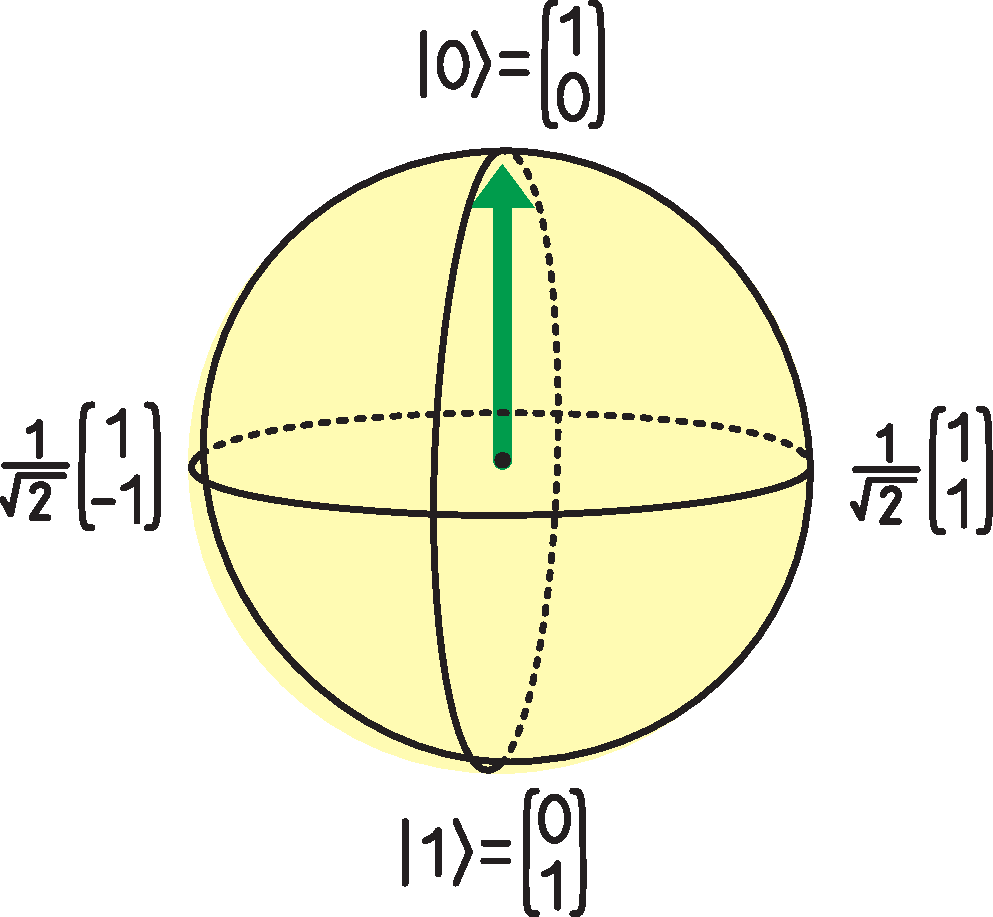
\includegraphics[width=\linewidth]{pdf/states/ground-state.pdf}
        \caption{Ground state.}
        \label{fig:Bloch-sphere-ground-state}
    \end{minipage}
    %
    \hfill
    %
    \begin{minipage}[t]{0.3\linewidth}
        \centering
        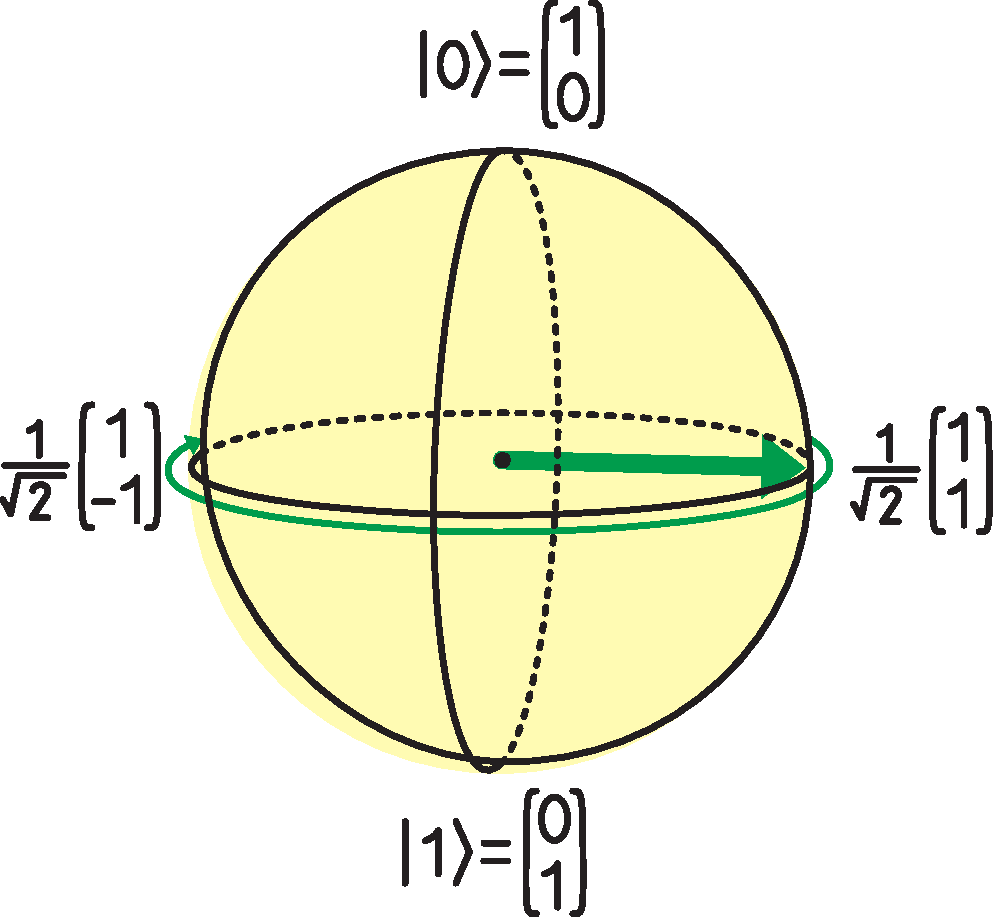
\includegraphics[width=\linewidth]{pdf/states/superposition-state.pdf}
        \caption{Superposition state.}
        \label{fig:Bloch-sphere-superposition}
    \end{minipage}
    %
    \hfill
    %
    \begin{minipage}[t]{0.3\linewidth}
        \centering
        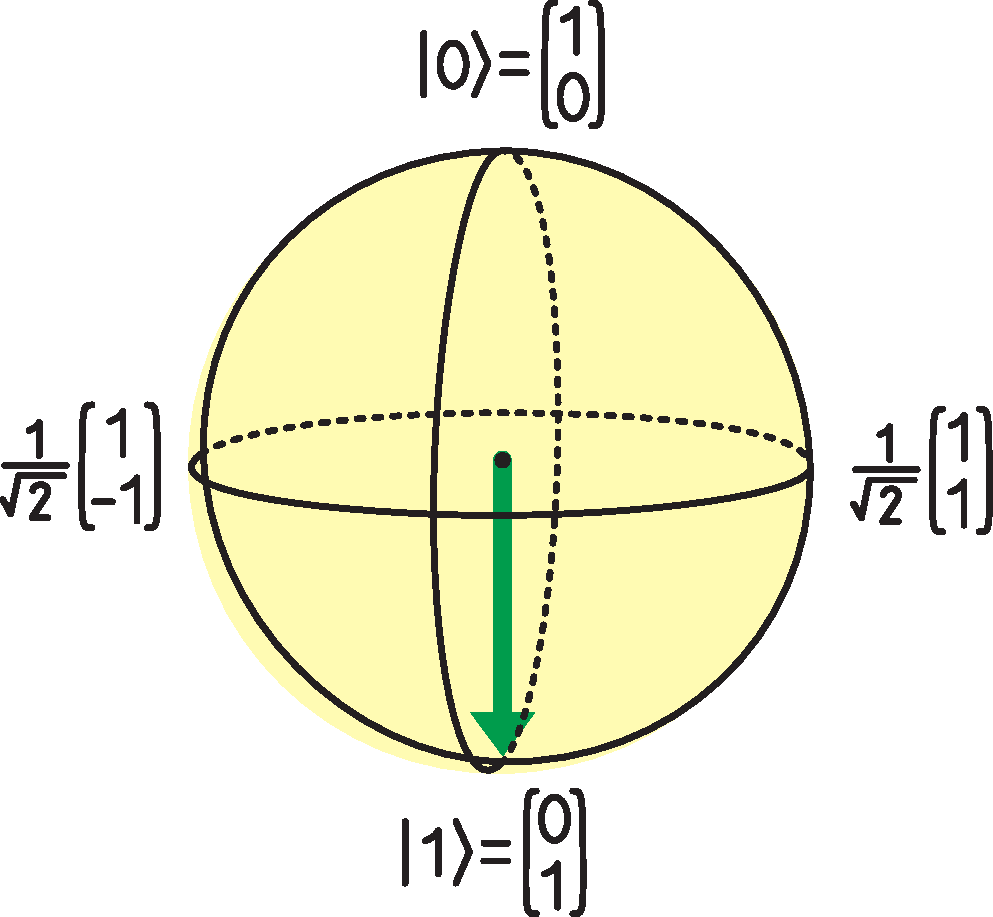
\includegraphics[width=\linewidth]{pdf/states/excited-state.pdf}
        \caption{Excited state.}
        \label{fig:Bloch-sphere-excited-state}
    \end{minipage}

    \caption{State superposition via Bloch sphere representation.}
    \label{fig:Bloch-sphere}
\end{figure}

\begin{figure}[H]
    \centering

    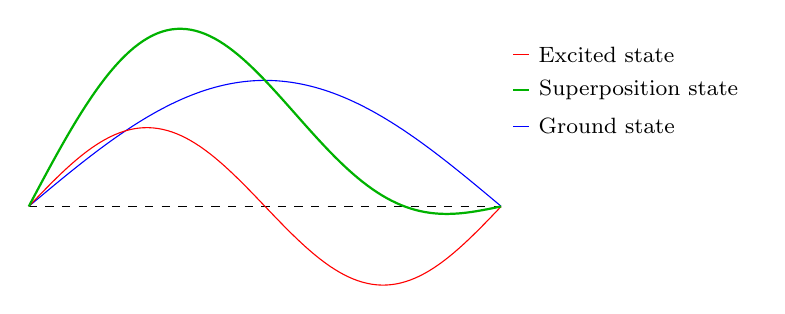
\begin{tikzpicture}

        \draw[dashed] (0, 0) -- (6, 0);

        \draw[blue, domain=0:6, samples=100] plot (\x, {1.6*sin(180/6*\x)});
        \draw[red, domain=0:6, samples=100] plot (\x, {1.0*sin(360/6*\x)});
        \draw[green!70!black, thick, domain=0:6, samples=100] plot (\x, {1.6*sin(180/6*\x) + 1.0*sin(360/6*\x)});

        % Add legend
        \node [matrix, font = \footnotesize, below right, row sep = 0cm] at (current bounding box.north east)
        {
            \draw[red] (0, 0) -- ++(0.2, 0) node[right, black] {Excited state}; \\
            \draw[green!70!black, thick] (0, 0) -- ++(0.2, 0) node[right, black] {Superposition state}; \\
            \draw[blue] (0, 0) -- ++(0.2, 0) node[right, black] {Ground state}; \\
        };

    \end{tikzpicture}

    \caption{State superposition via modal interpretation and wave functions.}
    \label{fig:modal-superposition}
\end{figure}


\paragraph{$\Lambda$-Lambda System \& Dark State}

We can proceed and understand how the states' superposition is used related to the operation of a \acrshort{cpt}-based \acrshort{csac}.
To do so, we need to introduce the concepts of $\Lambda$-Lambda system and dark state.

A $\Lambda$-Lambda system is a quantum system composed of three energy levels (see Figure \ref{fig:lambda-system} for reference), where not all the dipole transitions are allowed.
In particular:

\begin{figure}[H]
    \centering

    \begin{minipage}[c]{0.49\linewidth}
        \centering
        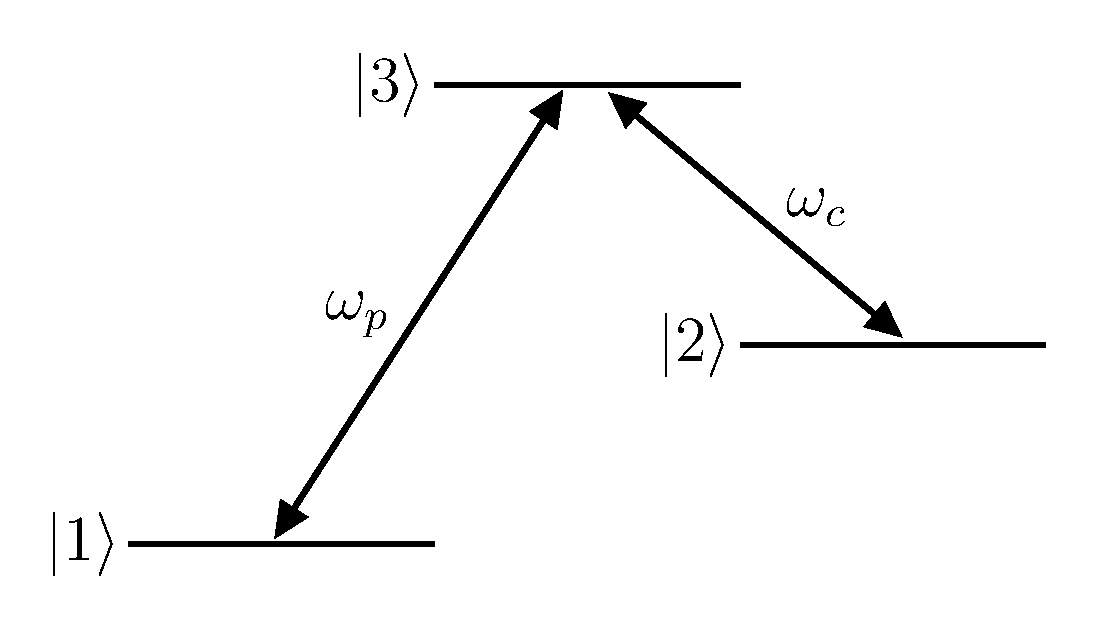
\includegraphics[width=\textwidth, max width=\linewidth]{pdf/lambda-system.pdf}
        \caption{$\Lambda$-system representation. Source \cite{LambdaSystem}.}
        \label{fig:lambda-system}
    \end{minipage}
    %
    \hfill
    %
    \begin{minipage}[c]{0.49\linewidth}
        \begin{align}
            \text{Allowed transitions:}  & \begin{cases}
                                               \ket{1} \leftrightarrow \ket{3} \\
                                               \ket{2} \leftrightarrow \ket{3}
                                           \end{cases} \\
            \text{Forbidden transition:} & \begin{cases}
                                               \ket{1} \leftrightarrow \ket{2}
                                           \end{cases}
        \end{align}
    \end{minipage}

\end{figure}


In case the system is excited with a stable and well-controlled laser source (more comprehensive explanation given in the following paragraph) that couples at the same time both $\ket{1} \leftrightarrow \ket{3}$ and $\ket{2} \leftrightarrow \ket{3}$ transitions, electrons will be pumped at first in their excited state (i.e. $\ket{3}$) and then forced to decay to $\ket{\psi}$, a superposition of $\ket{1}$ and $\ket{2}$.
This method is called \textit{coherent population trapping} and the system is said to be in a \textit{dark state} given that the incoming laser source will no more be coupled with the electron transitions and the atoms will not absorb the photons.

In our working frame, the $\Lambda$-system is composed of the two ground states $6^2S_{1/2} F=3$ \& $6^2S_{1/2} F=4$ and the excited state $6^2P_{1/2}$ of the $^{133}Cs$ atom.


\paragraph{Pumping Source}

From now on, given for granted the concept of quantum superposition and $\Lambda$-system, we can step into understanding the components used to excite the $^{133}Cs$ atoms and obtain the desired dark state.

In a \acrshort{cpt}-based \acrshort{csac}, the pumping source is typically a \textit{diode laser} (see Figure \ref{fig:CPT-physics-package-scheme} for reference), and most commonly a \textit{Vertical Cavity Surface Emitting Laser (VCSEL)}.
The use of a diode laser instead of a bulb lamp is due to the need of a stable and well-controlled source of irradiation that can be precisely modulated based on the local oscillator frequency.
In fact, VCSEL is a semiconductor laser diode that emits light from its top surface and it's characterized by a very narrow emission spectrum and a high modulation bandwidth.

In the framework of \acrshort{csac}, the diode laser is driven by the local oscillator frequency and it's modulated in both Amplitude (AM) and Frequency (FM).
In particular, in order to obtain the desired effect of coherent population trapping inside the reference cell, the laser source must met the following requirements:

\begin{itemize}
    \item AM modulation: the signal generated via the AM modulation must be at half the \ref{itm:Cs-I} frequency (i.e. half the transition frequency of the $^{133}Cs$ ground states hyperfine splitting);
    \item FM modulation: the signal generated via the FM modulation must be at frequency of the \textit{D1 line} (i.e. the transition frequency of the $^{133}Cs$ ground state to the $^{133}Cs$ excited state).
    \item Circular polarization: the laser source must be positively circularly polarized.
\end{itemize}

The first two requirements can be easily met by controlling the injection current of the diode laser in time and are equivalent to state that the laser source must be the sum of a signal modulated at \ref{itm:Cs-II} with another modulated at \ref{itm:Cs-III} frequency.
In other words, the laser source must be able to generate the beating wave of the two frequencies as shown in Figure \ref{fig:beating-wave}.
The third requirement can be met by using a quarter-wave plate in front of the laser source that convert the linear polarization of the source in a circular one (again, see Figure \ref{fig:CPT-physics-package-scheme} for reference).

\begin{figure}[H]
    \centering

    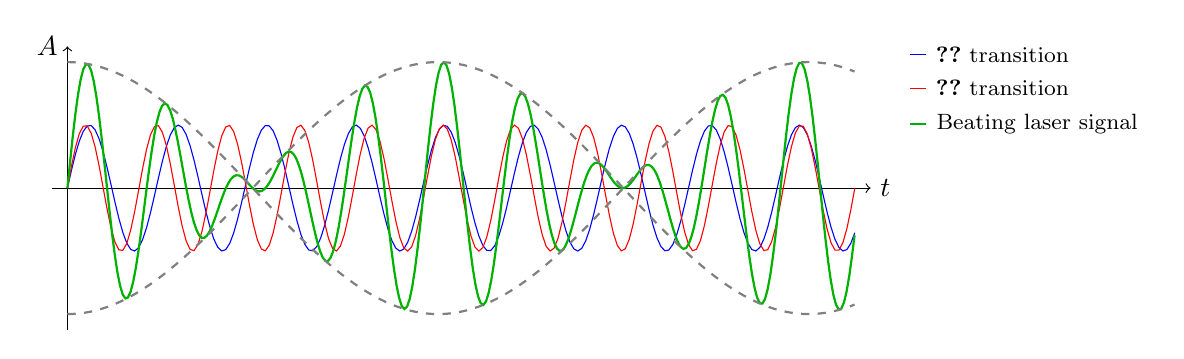
\begin{tikzpicture}
        \def\fa{1.775/2}
        \def\fb{2.20/2}
        \def\xmax{10}

        \draw[->] (-0.2, 0) -- (\xmax + 0.2, 0) node[right] {$t$};
        \draw[->] (0, -1.8) -- (0, 1.8) node[left] {$A$};

        \draw[blue, domain=0:\xmax, samples=200] plot (\x, {0.8*sin(360*\fa*\x)});
        \draw[red, domain=0:\xmax, samples=200] plot (\x, {0.8*sin(360*\fb*\x)});
        \draw[green!70!black, thick, domain=0:\xmax, samples=300] plot (\x, {0.8*sin(360*\fa*\x) + 0.8*sin(360*\fb*\x)});
        \draw[gray, thick, dashed, domain=0:\xmax, samples=300] plot(\x,{ 1.6*cos(180*(\fa-\fb)*\x)});
        \draw[gray, thick, dashed, domain=0:\xmax, samples=300] plot(\x,{ -1.6*cos(180*(\fa-\fb)*\x)});

        % Add legend
        \node [matrix, font = \footnotesize, below right, row sep = 0cm] at (current bounding box.north east)
        {
            \draw[blue] (0, 0) -- ++(0.2, 0) node[right, black] {\ref{itm:Cs-II} transition}; \\
            \draw[red] (0, 0) -- ++(0.2, 0) node[right, black] {\ref{itm:Cs-III} transition}; \\
            \draw[green!70!black, thick] (0, 0) -- ++(0.2, 0) node[right, black] {Beating laser signal}; \\
        };

    \end{tikzpicture}

    \caption{Beating wave of the laser source in a CPT-based \acrshort{csac} (AM modulation is highlighted with a dashed gray line, FM modulation is clearly visible on the green wave).}
    \label{fig:beating-wave}
\end{figure}

Notice, however, that the one represented in Figure \ref{fig:beating-wave} is the ideal case where the laser source is perfectly modulated at the two frequencies \ref{itm:Cs-II} and \ref{itm:Cs-III}.
In reality, the laser source is driven by the local oscillator frequency and some modulation errors will appear.
Those shift with respect to the ideal case will give us the information needed to understand if the local oscillator is in resonance with the atomic transition or not.

\paragraph{Electrons Excitation and Interrogation}

Having explained the requirements of the excitation source, we can now proceed understanding how this energy is used over the atoms present in the \textit{reference cell} (see Figure \ref{fig:CPT-physics-package-scheme}, also refereed to as \textit{vapor gas cell}) and in particular what's the cycle that electrons are forced to.

For the simplicity of the explanation, we will consider the different stages of the electrons as if they happen in a temporal sequence.
However, it's important to remind those stages are not sequential but they happen simultaneously.

We can define three different stages in the cycle of the electrons:

\begin{itemize}
    \item Optical pumping (population inversion): the laser source coming from the diode laser excites the atoms from both the $6S_{1/2} F=3$ and the $6S_{1/2} F=4$ ground hyperfine states to the $6^2P_{1/2}$ excited state.
    \item Decay to the dark state (superposition state): if the laser source during the pumping stage wss modulated properly as described in the previous paragraph, then the excited electrons will now decay to a coherent superposition of the two ground states $6S_{1/2} F=3$ and $6S_{1/2} F=4$. The atoms are now in a dark state.
    \item Optical pumping (interrogation): the same laser used for population inversion is now used to interrogate the atoms and understand if the local oscillator frequency was in resonance with the atomic transition \ref{itm:Cs-I} or not.
\end{itemize}

To visualize the cycle of the electrons, we can refer to Figure \ref{fig:CPT-steps}.

\begin{figure}[H]
    \centering

    \begin{minipage}[t]{0.3\linewidth}
        \centering
        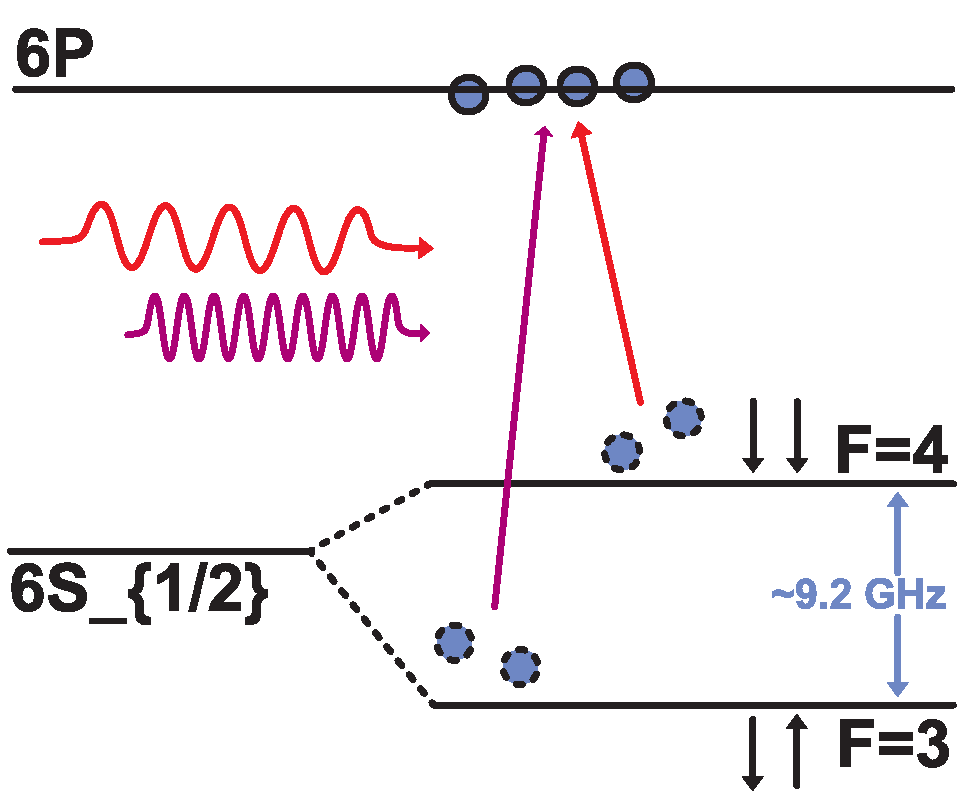
\includegraphics[width=\linewidth]{pdf/CPT/pumping.pdf}
        \caption{Population inversion.}
        \label{fig:CPT-pumping}
    \end{minipage}
    %
    \hfill
    %
    \begin{minipage}[t]{0.3\linewidth}
        \centering
        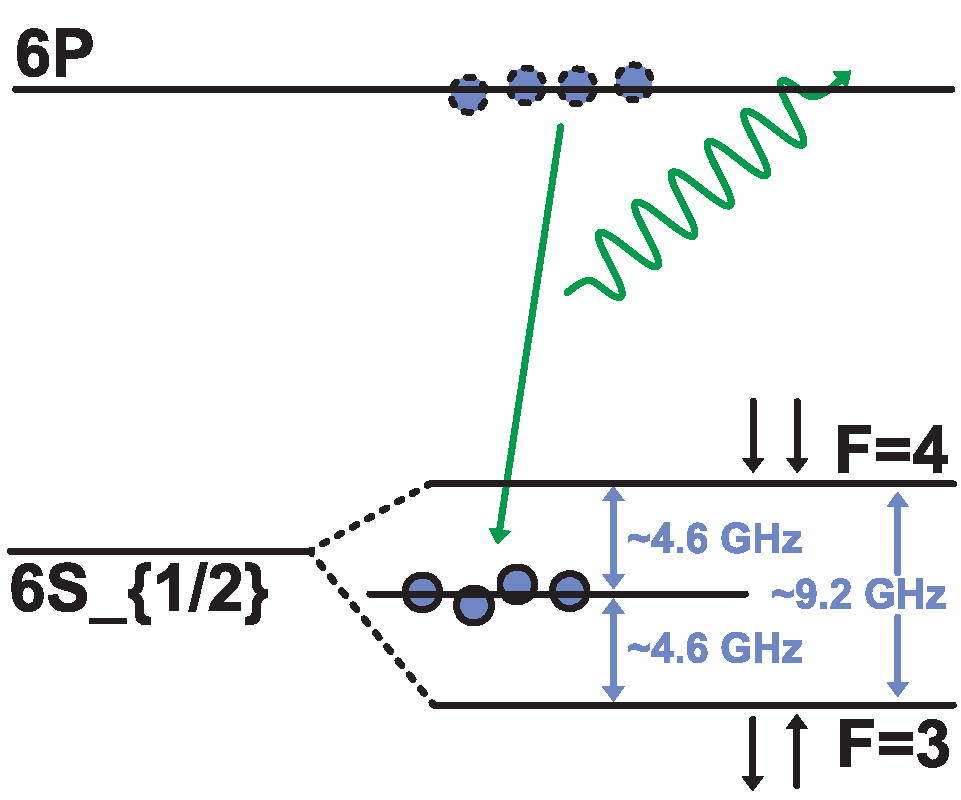
\includegraphics[width=\linewidth]{pdf/CPT/decay.pdf}
        \caption{Population decay.}
        \label{fig:CPT-decay}
    \end{minipage}
    %
    \hfill
    %
    \begin{minipage}[t]{0.3\linewidth}
        \centering
        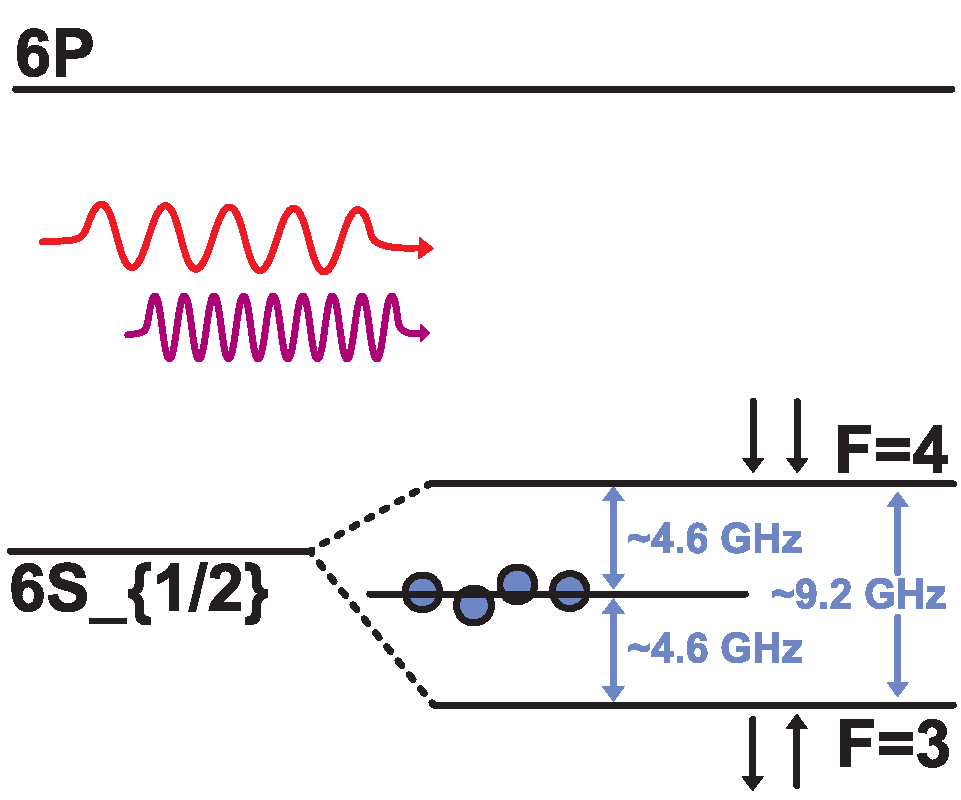
\includegraphics[width=\linewidth]{pdf/CPT/interrogation.pdf}
        \caption{Optical interrogation.}
        \label{fig:CPT-interrogation}
    \end{minipage}

    \caption{Electrons cycle in a CPT-based \acrshort{csac} due to the optical pumping, decay and optical interrogation.}
    \label{fig:CPT-steps}
\end{figure}

For the sake of the explanation and simplification, we will consider the pumping laser source (the one coming from the diode laser) as two separate signals, one modulated at the frequency \ref{itm:Cs-II} and the other modulated at \ref{itm:Cs-III}, even if in reality a single beating wave of the two frequencies is used (Figure \ref{fig:beating-wave}).

In Figure \ref{fig:CPT-pumping}, we can see four electrons that get excited from $6S_{1/2} F=3$ and $6S_{1/2} F=4$ ground hyperfine states to the $6^2P_{1/2}$ excited state.

Being $6^2P_{1/2}$ an unstable state, electrons will start to decay to the non-excited states.
In Figure \ref{fig:CPT-decay}, we can see that over time the population will tend to accumulate in a coherent superposition of the two ground states, given that from here the electrons won't be coupled to the laser source anymore.
Notice, however, that the accumulation in the superposition state is possible only if the laser source was properly modulated, that is equivalent to say that the local oscillator was in resonance with the atomic transition \ref{itm:Cs-I}.

Finally, the cycle is closed with the interrogation phase (Figure \ref{fig:CPT-interrogation}).
Here, by sending the same amount of irradiation as in the pumping phase, we are able to detect if electrons are in the superposition state or not.
In Figure \ref{fig:CPT-interrogation}, we can see that all the electrons are found in the superposition state and so the intensity of the transmitted light will be maximal since none of those electrons is coupled with the laser source.

By measuring the intensity of the transmitted light, we can understand if the local oscillator was in resonance with the atomic transition or not.


\paragraph{Photodetector}

At the end of the reference cell, a photodetector is used to measure the intensity of the transmitted light.

In case of a CPT-based \acrshort{csac}, given that if the microwave signal was in resonance with the atomic transition, most of the electrons are now in the dark state, then the intensity of the transmitted light will be maximal.
Conversely, in case of a non-resonant microwave signal, the intensity of the transmitted light will be lower (a fraction of the light will be absorbed by electrons that are not in the dark state).
In Figure \ref{fig:CPT-transmission}, we can see an example of a detuned signal captured by the photodetector.

\begin{figure}[H]
    \centering
    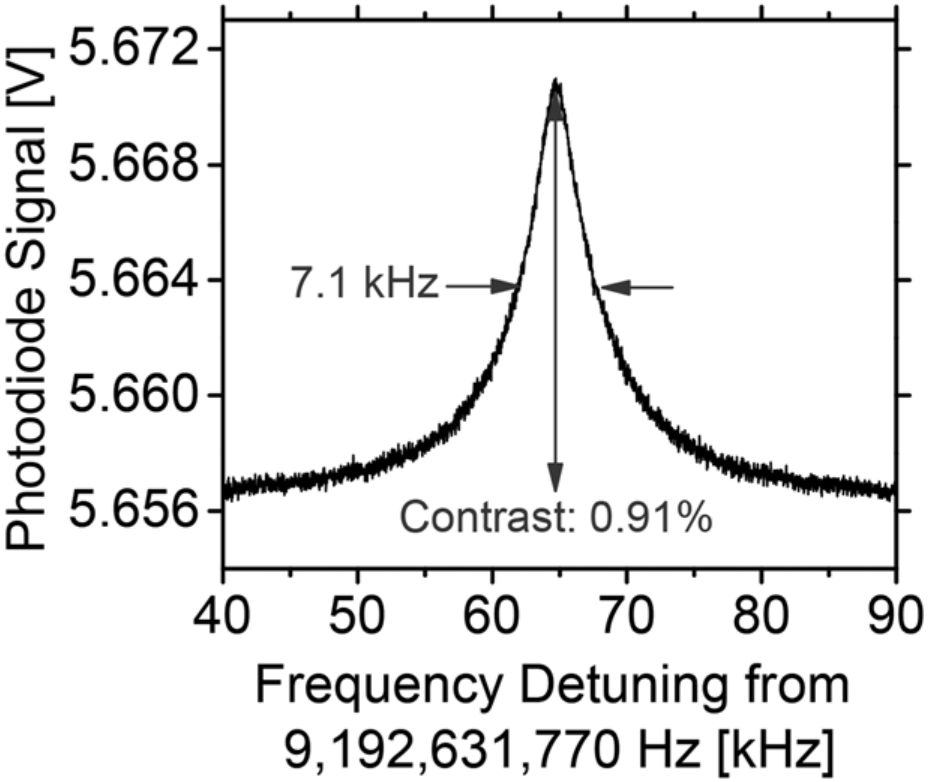
\includegraphics[width=0.5\textwidth, max width=0.8\linewidth]{img/CPT-transmission-signal.png}
    \caption{Detuned photodetection signal in a CPT-based \acrshort{csac}. Source \cite{Kitching-2018}.}
    \label{fig:CPT-transmission}
\end{figure}

The signal captured by the photodetector is then sent to the control loop that will use it to fine-tune the local oscillator frequency.

